\chapter{Saliency Maps}
\label{cha:saliency}
Das \textit{Saliency Map} Verfahren wurde erstmals von den Neurowissenschaftlern Itti et al. \cite{itti_model_1998} in ihrer Studie vorgeschlagen. 
Die Studie beschreibt eine Methode zur Extraktion von einzigartigen Merkmalen, wie beispielsweise Farben, Farbintensitäten und Strukturen, sogenannten High-Level Features, aus Bildern, die wiederum in sogenannten \textit{Saliency Maps} topografisch visualisiert werden. 
Diese High-Level Features sind nichts anderes als spezifische Pixel im Bild auf Mikroebene (Low-Level Features), welche die optisch ansprechendsten respektive bedeutendsten Stellen in einem Bild repräsentieren \cite{itti_model_1998}. 

Um also spezifischen Bildmerkmalen eine semantische Bedeutung zuzuordnen, werden beispielsweise Farbbilder anhand des \textit{Saliency Map}-Verfahrens in Schwarzweißbilder umgewandelt, um die stärksten darin vorhandenen Farben zu analysieren und extrahieren.

\section{Konzept}
\label{cha:saliency_konz}
Bei \ac{CNN} werden Merkmale von Eingabebildern extrahiert, indem zunächst im Input-Layer Low-Level Features, und mit jeder weiteren Schicht des Netzwerks immer komplexere Merkmale (High-Level Features), wie etwa Kanten, Rundungen oder Strukturen erlernt werden \cite{stanford_unsupervised_tutorial}.

Diese Kenntnis um \ac{CNN} und \textit{Saliency Maps} machten sich Simonyan et. al erstmalig im Kontext von Deep Learning zunutze, um die gelernten Merkmale eines \ac{CNN} anhand von \textit{Saliency Maps} zu visualisieren \cite{simonyan_deep_2013}. 
Die in der Arbeit von Simonyan et. al erzeugten Bilder sind hierbei nicht oder nur ansatzweise für den Menschen erkennbar, wurden jedoch vom zugrunde liegenden \ac{CNN} mit einer hohen Konfidenz richtig klassifiziert.
~\newline

Aus dieser Kenntnis ergeben sich folgende Hypothesen:
\begin{itemize}
	\item Ein Convolutional Neural Network mit beliebiger Architektur, jedoch trainiert mit demselben Datensatz (\ac{GTSRB}) wie das \ac{NN} des \ac{GI}-Wettbewerbs, lässt sich ähnlich gut angreifen wie das \ac{NN} des \ac{GI}-Wettbewerbs selbst. Zu dieser Erkenntnis kamen Papernot et al. \cite{papernot_+_2016} im Rahmen ihrer Arbeit. 
	Auf diesen Sachverhalt wird in Kapitel \ref{sec:TrasiModell} näher eingegangen.
	\item 	\textit{Saliency Maps} repräsentieren die wesentlichen Merkmale, die das Convolutional Neural Network zu den Eingabebildern gelernt hat. 
	Die erzeugten Bilder mit dem \textit{Saliency Map} Verfahren werden wiederum vom \ac{CNN} mit einer hohen Konfidenz richtig klassifiziert. 
	Das heißt, dass jeweils erzeugte Bild wird vom \ac{CNN} als Verkehrszeichen erkannt und mit hoher Konfidenz richtig klassifiziert, ist jedoch für den Menschen nicht als solches erkennbar.
\end{itemize}
Werden diese Hypothesen erfüllt, so eignet sich das Verfahren der \textit{Saliency Maps} ebenfalls zur erzeugung von \textit{Adversarial Attacks}
\section{Implementierung}

Als vorverarbeitenden Schritt werden zunächst alle 12.630 Bilder aus dem GTSRB-Testdatensatz, welche in 24-Bit Farbtiefe und im \ac{PPM} Dateiformat vorliegen, in das \ac{PNG} Dateiformat konvertiert und im Dateisystem abgespeichert. 
Die vorliegenden PNG-Bilder werden anhand des \textit{Aphrodite}-Modells, auf dessen Architektur und Training in Kapitel \ref{sec:ImplAphrodite} eingegangen wird, klassifiziert: 
Nur diejenigen Bilder, welche vom \textit{Aphrodite}-Modell mit einer Konfidenz von 100\% korrekt klassifiziert wurden (3.063/12.630) werden im Dateisystem in einem eigenständigen Verzeichnis abgespeichert.

Gemäß einer auf die Anforderungen an die Aufgabenstellung abgewandelten Variante zu Anh \cite{anh_implementations_2019}, erfolgt nun die Implementierung der verschiedenen \textit{Saliency Map}-Verfahren.

~\newline Hierzu werden zunächst die Basismethoden \textit{Vanilla} \cite{simonyan_deep_2013}, \textit{Guided Backpropagation} \cite{springenberg_striving_2014} und \textit{Integrated Gradient} \cite{sundararajan_axiomatic_2017} implementiert. 

Unter Verrauschung, gemäß \cite{smilkov_smoothgrad:_2017}, werden die Basismethoden verbessert, wie die Gegenüberstellung der Ergebnisse zu den eingesetzten Verfahren in Kapitel \ref{sec:SalErgebnisse} verdeutlicht.

Diese optimierten Varianten werden als \textit{Smoothed Vanilla}, \textit{Smoothed Guided Backpropagation} und \textit{Smoothed Integrated Gradient} bezeichnet und implementiert.

Jedes der \textit{Saliency Map}-Verfahren wird auf die mit dem \textit{Aphrodite}-Modell klassifizierten Bilder angewendet.
Diese Bilder werden nacheinander vom Dateisystem geladen und anschließend auf eine Zielbildgröße von $64 \times 64 $ Pixel interpoliert. 
Das \textit{Saliency Map}-Verfahren extrahiert nun die vom zugrunde liegenden Modell (Aphrodite) gelernten Merkmale. 
Hierzu wird das jeweilige Eingabebild und das Aphrodite Modell verwendet. 
Die damit erzeugten Bilder werden anschließend in einem gesonderten Verzeichnis in der Größe $64 \times 64 $ Pixel im Dateisystem abgespeichert.


Zur abschließenden Evaluierung der erzeugten Bilder am \ac{NN} des \ac{GI}-Wett"-be"-werbs, werden alle Bilder zu jedem eingesetzten \textit{Saliency Map} Verfahren im Zyklus von 60 Bildern pro Minute an das Webinterface des Wettbewerbs gesendet. 
Die Informationen, das heißt die vom \ac{NN} des \ac{GI}-Wettbewerbs erkannte Zielklasse und Konfidenz, werden anschließend aus dem HTTP-Response"-code zu jedem übermittelten Bild in zwei verschiedenen Logdateien gespeichert: 
Die erste Logdatei speichert alle Ergebnisse aus dem jeweiligen HTTP-Response"-code, wohingegen die zweite Logdatei nur Ergebnissemit über 90\% Konfidenz, zu den übermittelten Bildern enthält.

\section{Ergebnisse}
\label{sec:SalErgebnisse}
Mit den verschiedenen \textit{Saliency Map} Verfahren wurden Graustufenbilder erzeugt, in denen die relevanten Bildmerkmale durch helle Pixeleinfärbungen gekennzeichnet sind. 

Die mit den Basismethoden \textit{Vanilla}, \textit{Guided Backpropagation} und \textit{Integrated Gradient} erzeugten Bilder werden vom \ac{NN} des \ac{GI}-Wettbewerbs mit jeweils 45,83\% als "`Baustelle"' klassifiziert.

Dieses Ergebnis lässt sich möglicherweise auf die besonderen "`Faltungseigenschaften"' von Convolutional Neural Networks zurückführen, dass bildcharakterisierende Merkmale und die verbundene semantische Information aus den erzeugten Bildern verloren ging.

Mit den optimierten \textit{Saliency Map} Verfahren (\textit{Smoothed Vanilla}, \textit{Smoothed Guided Backpropagation} und \textit{Smoothed Integrated Gradient}) Bilder erzeugt werden, die Zielkonfidenzen von mehr als 90\% am \ac{NN} des \ac{GI}-Wettbewerbs erreichten.

\begin{table}
	\centering
	\begin{tabular}{p{4.5cm}p{4.5cm}p{4.5cm}}
		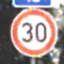
\includegraphics[width=\linewidth]{Images/AnPe/5_1_Links} & 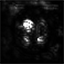
\includegraphics[width=\linewidth]{Images/AnPe/5_1_Mitte} &
		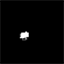
\includegraphics[width=\linewidth]{Images/AnPe/5_1_Rechts}\\ 
		5.1a: Ursprungsbild &5.1b: Smoothed Guided Backprop. &5.1c: Smoothed Vanilla Saliency \\
		30ger Zone & Allgemeines Überholverbot & 30ger Zone\\
		99,39\% Konfidenz & 91,55\% Konfidenz & 92,83\% Konfidenz\\
		
	\end{tabular} 

	\caption{Ergebnisse der Verfahren Smoothed Guided Backpropagation und Smoothed Vanilla Saliency}
	\label{tab:sal1}
\end{table}

Tabelle \ref{tab:sal1} zeigt exemplarisch, wie aus dem Ursprungsbild (5.1a "30ger Zone"'), unter Verwendung des \textit{Smoothed Guided Backpropagation} Verfahrens, ein Bild erzeugt wurde, das vom \ac{NN} des \ac{GI}-Wettbewerbs mit 91,55\% als "`Überholverbot"' klassifiziert wurde (5.1b). 
Das \textit{Smoothed Vanilla Saliency} Verfahren erzeugte hingegen aus demselben Ursprungsbild ein Bild, das mit einer Zielkonfidenz von 92,83\% vom \ac{NN} des \ac{GI}-Wettbewerbs als "`30ger Zone"' erkannt wurde (5.1c).

Tabelle \ref{tab:sal2} zeigt weitere Beispiele für erfolgreiche Bilder, unter Verwendung der optimierten \textit{Saliency Map}-Verfahren. 
Wieder kann beobachtet werden, dass die erzeugten Bilder zwar mit einer Zielkonfidenz von über 90\% vom \ac{NN} des \ac{GI}-Wettbewerbs klassifiziert wurden, die ursprüngliche Klasse jedoch abweicht.

\begin{table}
	\centering
	\begin{tabular}{p{7,5cm}p{7cm}}
		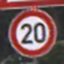
\includegraphics[height=4.4cm]{Images/AnPe/5_2_Oben-links} & 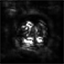
\includegraphics[height=4.4cm]{Images/AnPe/5_2_Oben_rechts} \\
		Ursprungsbild: & Smoothed Guided Back"-propagation:\\
	 	20ger Zone & Allgemeines Überholverbot\\
		97,54\% Konfidenz & 97,63\% Konfidenz\\
		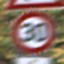
\includegraphics[height=4.4cm]{Images/AnPe/5_2_Mitte-links} &
		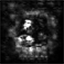
\includegraphics[height=4.4cm]{Images/AnPe/5_2_Mitte_rechts}  \\
		Ursprungsbild: & Smoothed Guided Back"-propagation:\\
		30ger Zone & 50ger Zone\\
		66,07\% Konfidenz & 99,94\% Konfidenz\\
		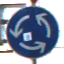
\includegraphics[height=4.4cm]{Images/AnPe/5_2_Unten_links} &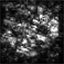
\includegraphics[height=4.4cm]{Images/AnPe/5_2_Unten_rechts}  \\
		Ursprungsbild: & Smoothed Integrated Gradient:\\
		Kreisverkehr & Baustelle\\
		93,92\% Konfidenz & 99,99\% Konfidenz\\
	\end{tabular}
	\caption{Ergebnisse Smoothed Guided Backpropagation und Smoothed Integrated Gradient}
\label{tab:sal2}
\end{table}

Zusammenfassend konnte hiermit gezeigt werden, dass die in Kapitel \ref{cha:saliency_konz} formulierten Hypothesen zutreffen und sich Bilder – unter Verwendung eines eigens trainierten \ac{CNN} Modells (\textit{Aphrodite}) sowie verschiedener \textit{Saliency Map} Verfahren – erzeugen lassen, die zwar keine für den Menschen sinnvolle Bedeutung haben, jedoch beim \ac{NN} des \ac{GI}-Wettbewerbs Zielkonfidenzen von mehr als 90\% erreichten.